\section{LoRa}\label{sec:etat_art-lora}
\renewcommand{\rightmark}{LoRa}

LoRa (Long Range) est une technologie radio  fonctionnant sur une modulation radio propriétaire
détenue par Semtech. Cette modulation est dérive de la modulation \textit{chirp spread spectrum (CSS)} et permet d'obtenir des communications longues portées\todo{chiffres} et basses énergie.

\begin{wrapfigure}{r}{0.3\textwidth}
    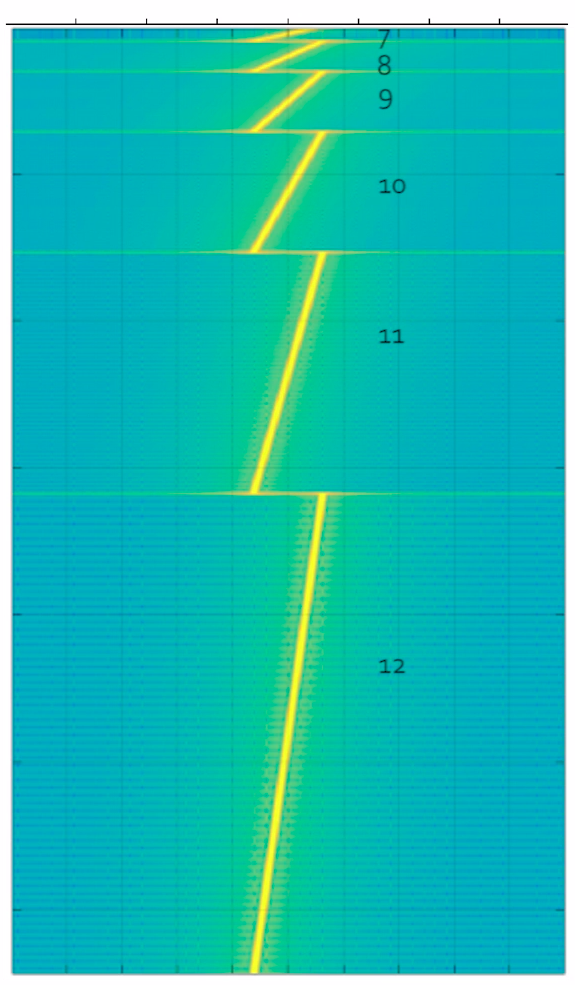
\includegraphics[scale=0.25]{res/pictures/lora-sf.png}
    \caption{Signal en fonction du SF.\todo{ref}}
    \label{fig:state-sf}
\end{wrapfigure}
Une communication LoRa dépend des paramètres suivants:
\begin{itemize}
    \item \textbf{Spreading Factor (SF)}: SF est une variable qui définit la vitesse de balayage du signal radio (Fig~\ref{fig:state-sf}). Le spreading factor est compris entre 7 et 12. Plus la valeur est grande, plus la vitesse de balayage est petite et donc le signal est plus facile à décoder. mais le débit des données est plus faible. Donc une grande valeur de SF implique un débit plus faible mais une QoS (Quality of Service) plus élevée et inversemment pour une petite valeur de SF.
    \item \textbf{Bandwidth (BW)}: Détermine la largeur de la bande passante. Une bande passante plus large augmente la qualité du signal. Pour LoRa, en Europe les valeurs de BW sont limitées à 125 KHz et 250KHz.\todo{ref thethingsnetwork}
    \item \textbf{Coding rate (CR)}:
\end{itemize}

\vspace{1cm}
Le format des paquets LoRa(Fig.~\ref{fig:state-lora-frame-format}) peut être explicite ou implicite.
Dans le mode implicite, le header n'est pas inclus dans le paquet. Pour cela, la taille de la payload, le coding rate et la présence de la Payload CRC doit être configuré 
Ce mode permet de réduire la taille du paquet et donc du temps de transmission.

\begin{figure}[H]
    \centering
    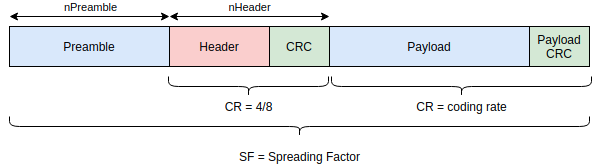
\includegraphics[scale=0.6]{res/pictures/lora-frame-format.drawio.png}
    \caption{Format d'un paquet LoRa.}
    \label{fig:state-lora-frame-format}
\end{figure}
%Le format des paquets LoRa est illustré à la figure~\ref{fig:state-lora-frame-format}. 
